\section{Path Planning using Reinforcement Learning}

This section covers the development of a reinforcement learning model to plan the path of a robot manipulator in a collaborative cell. The model was trained and tested in a simulated environment and then a small integration with the real collaborative cell was done to test the model in a real environment. All the code developed for this research is available in the following repository: \url{https://github.com/lardemua/rl-robot-control}.

\subsection{Simulated Environment}

The environment used for model training was based on the Fetch Reach environment made available by Gymnasium Robotics\footnote{Fetch Reach Environment from Gymnasium Robotics: \url{https://robotics.farama.org/envs/fetch/reach/}}. In this environment, the task was to make the manipulator move the end-effector to a random 3D position above a table in front of the robot, as show in \autoref{fig:fetch_reach_env}. The robot in this simulation has 7-DoF and is controlled by small displacements of the gripper in cartesian coordinates, with Mujoco being responsible for the inverse kinematics computation. This environment also forced the end-effector to always be facing downwards which is not always the case in a real collaborative environment.

\begin{figure}[H]%[ht]
    \centerline{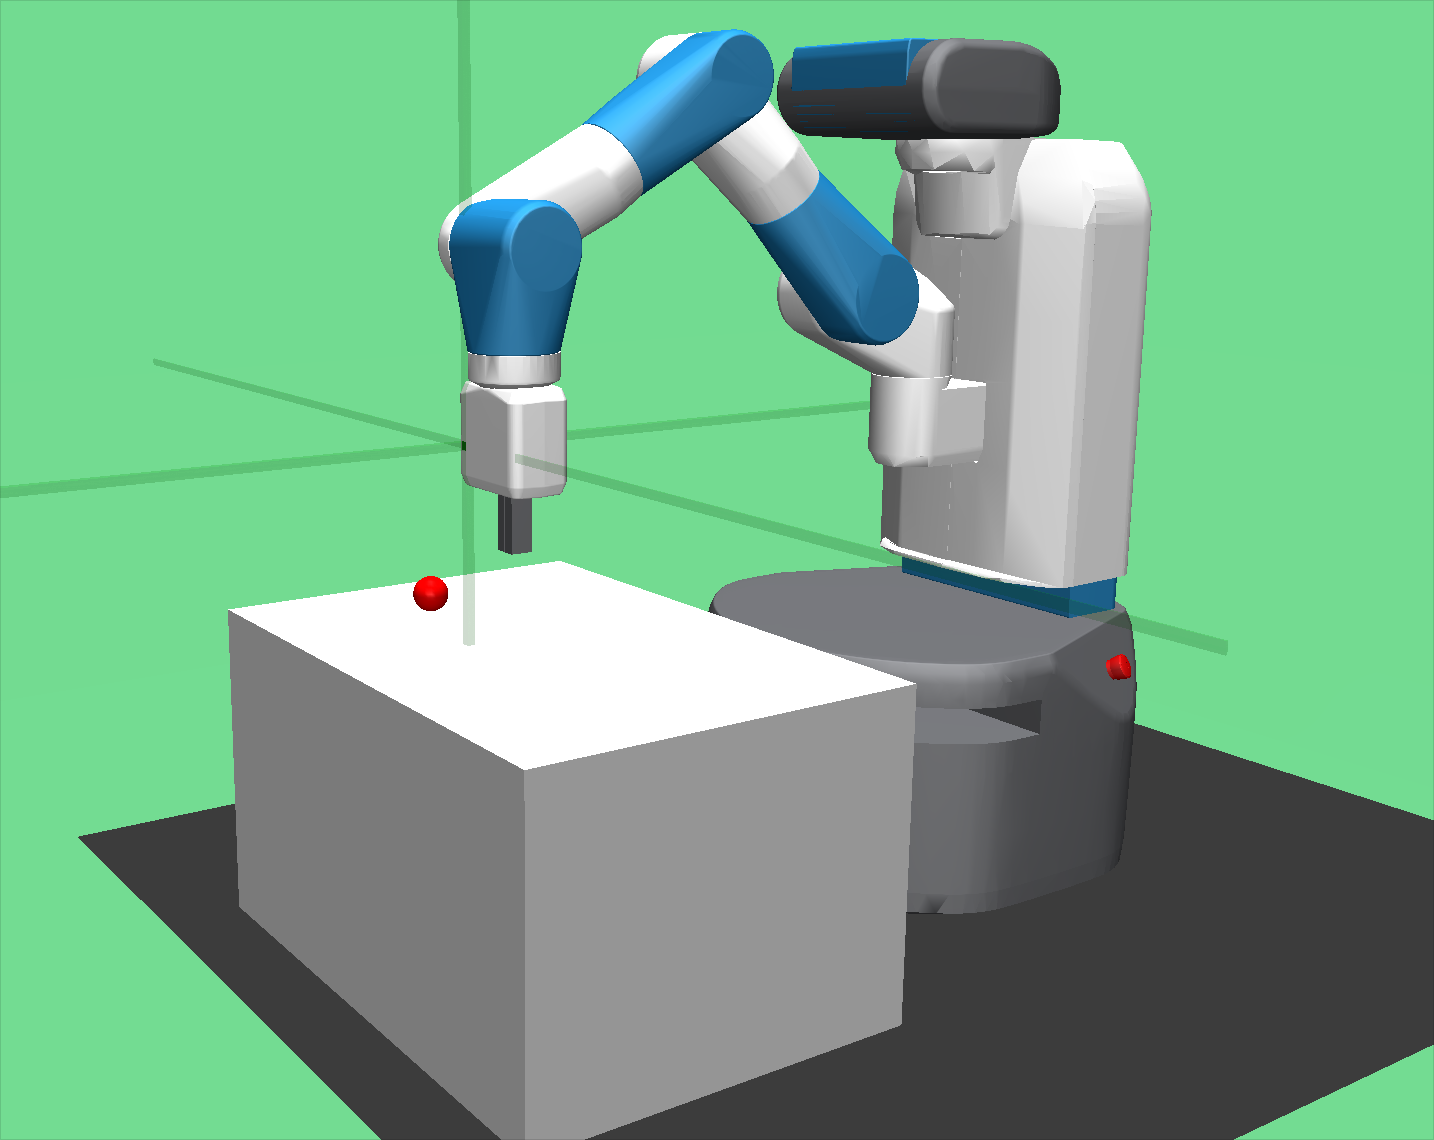
\includegraphics[width=0.7\textwidth]{figs/fetch_reach.png}}
    \caption[Fetch Reach Environment]{Fetch Reach Environment}
    \label{fig:fetch_reach_env}
\end{figure}

The Fetch Reach environment served as a starting point for this research but ended up being mostly rewritten to not only resemble the available collaborative cell but also allow for direct joint control instead of the previous cartesian displacements. The final environment, now named Larcc, can be seen in \autoref{fig:larcc_env} which now includes a UR10e robot model with a Robotiq 2F-140 gripper just like in the real collaborative cell. The UR10e model was obtained from Menagerie, a collection of models for Mujoco curated by Google DeepMind\footnote{UR10e Model from Menagerie: \url{https://github.com/google-deepmind/mujoco_menagerie/tree/main/universal_robots_ur10e}} while the gripper model was obtained from the robosuite framework by 
ARISE Initiative\footnote{Robotiq 2F-140 Model from robosuite: \url{https://github.com/ARISE-Initiative/robosuite/blob/master/robosuite/models/assets/grippers/robotiq_gripper_140.xml}}. The models used were edited so they could be used together, and the final environment was deemed acceptable given that the difference between the end-effector position in ROS and in the simulator differ by less than 1mm for the same joint positions. In this environment, the goal is to move the end-effector to a target position and orientation which are both represented by 3D axes in the simulator. As the actions affect the joints directly, a model trained is this environment ends up replacing the inverse or differential kinematics.

\begin{figure}[H]%[ht]
    \centerline{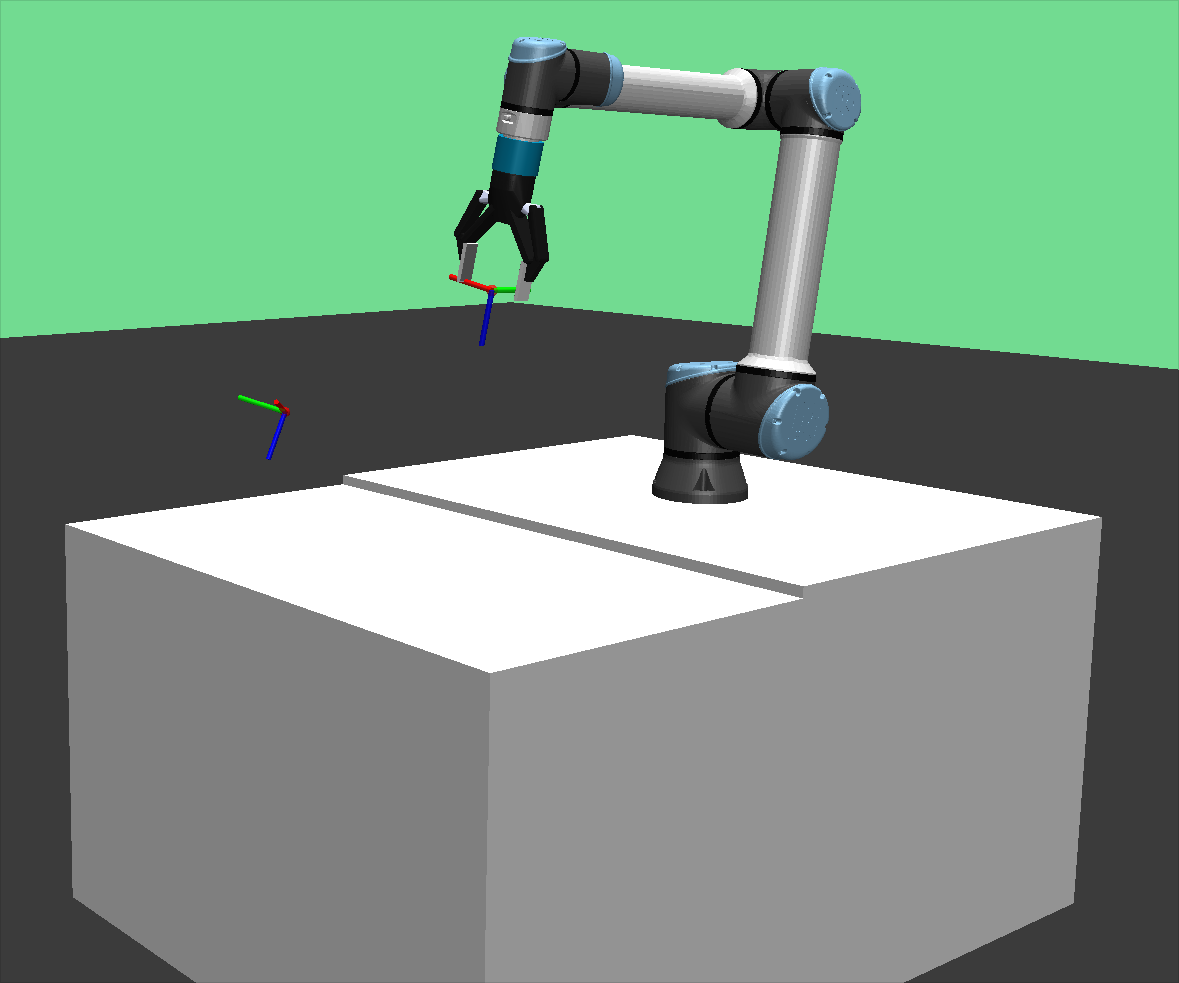
\includegraphics[width=0.7\textwidth]{figs/larcc_env.png}}
    \caption[Larcc Environment]{Larcc Environment}
    \label{fig:larcc_env}
\end{figure}

\subsubsection{Starting State}

To set up a new episode during training, the robot state and the goal position and orientation in the environment are reset.

For the goal, the position is sampled from a uniform distribution corresponding to the volume \SI{10}{\cm} to \SI{60}{\cm} above the table in front of the robot. The orientation is sampled from a uniform distribution in RPY format and then converted to quaternions. The orientation is then validated to check if it is facing mostly forward and downwards, which is the orientation that the gripper should have to pick up an object. If the orientation is not valid, a new one is sampled until a valid one is found.

For the starting state of the robot there are two possibilities: it can start in the fixed position shown in \autoref{fig:larcc_env} or in a random position. The random position is obtained by sampling the joint positions from a uniform distribution in the $[-\pi, \pi]$ interval, which is the same interval used for the joint limits in the UR10e robot. However, given that a fully random starting position can make the task too difficult, the end-effector position and orientation from the random starting position is validated with the same constraints as the goal position and a new starting position is sampled until a valid one is found.

\subsubsection{Observation Space}

The observation space in this environment follows the structure commonly used Gymnasium environments being a dictionary with 3 keys:

\begin{itemize}
    \item $observation$: consists of the positions of the 6 joints; given that they were limited to the $[-\pi, \pi]$ interval, they were normalized by a division by $\pi$;
    \item $achieved\_goal$: current position and orientation of the end-effector; the position was normalized by subtracting the position of the robot base link in the environment and then dividing by the arm's range, and the orientation was kept because it is defined with quaternions which are already in the $[-1, 1]$ interval;
    \item $desired\_goal$: position and orientation of the goal; normalized in the same way as the achived\_goal above.
\end{itemize}

\subsubsection{Action Space}

The action space represents the displacements in all joints for a single timestep. These displacements are also normalized which means that the final action applied to the environment is the result of the action output given by a model which is in the $[-1, 1]$ range multiplied by the maximum displacements of the joints. The first two joints associated with the shoulder can move at most 0.8 radians per timestep while the other four joints associated with the elbow and the wrist can move at most 1.2 radians per timestep, representing the different maximum velocities on the UR10e robot joints (https://www.universal-robots.com/products/ur10-robot/).

\subsubsection{Rewards}

The used environment has dense rewards so as to give the agent frequent and consistent feedback about its actions. This means that in every timestep the reward will increase if the the end-effector is closer to the goal and decrease otherwise, helping the model learn which actions lead to a successful episode. The reward in each timestep is obtained from the following rewards:

\begin{itemize}
    \item $position\_reward$: \[
            \begin{cases}
                1-distance(goal\_pos, end-effector\_pos) & \text{if $distance(...)<2$,}\\
                -1 & \text{otherwise}
            \end{cases};
        \]
    
    \item $orientation\_reward$: \[
            max\left(
            \begin{cases}
                innerproduct(goal\_quaternion, end$-$effector\_quaternion) \text{,}\\
                innerproduct(-goal\_quaternion, end$-$effector\_quaternion) 
            \end{cases}\right)\text{;}
        \]
    \item $bonus\_reward$: \[
            \begin{cases}
                1 & \text{if $position\_reward>0.98$ and $orientation\_reward>0.98$,}\\
                0 & \text{otherwise}
            \end{cases}\text{.}
        \]

\end{itemize}

\if{0}
\begin{itemize}
    \item $position$: \[1-distance(goal\_pos, end-effector\_pos), $if distance lower than 2$\],  otherwise $-1$ so that it is normalized;
    \item $orientation$: $max(, innerproduct(-goal\_quaternion, end$-$effector\_quaternion))$;
    \item $bonus$: $1$ if goal has been reached else $0$; the goal is considered reached if both the other rewards are above $0.98$.
\end{itemize}
\fi

These rewards affect the final timestep reward with different weights, but the sum of the weights is always equal to $1$ keeping the final reward in the $[-1, 1]$ range.

\subsection{Results}

The tests in the described environment were executed using the Soft Actor-Critic (SAC) algorithm. SAC is an off-policy model-free reinforcement learning algorithm known for its ability to achieve high performance while maintaining stability and sample efficiency. It is composed of three key components: an actor network, a critic network, and entropy regularization. The actor network is responsible for learning the policy and outputting the actions to be taken by the agent. The critic network is responsible for evaluating the actions taken by the agent. The entropy regularization is used to encourage exploration of the environment by introducing randomness or uncertainty in the agent's actions.

\subsubsection{Fixed Initial Position Results}

A SAC model was trained on the developed environment with a fixed initial robot state and with a $0.5$ weight on the position reward and a $0.25$ weight on the orientation and on the bonus reward. The model was trained with early stopping configured to evaluate the model every $500$ episodes and stop training if the evaluation average reward does not increase for $20$ evaluations. \autoref{fig:actor_loss} and \autoref{fig:critic_loss} show the evolution of the actor and critic loss during training.

\begin{figure}[H]%[ht]
    \centering
    {\fontsize{8}{11}\selectfont\includesvg[width=\textwidth]{figs/actor_loss.svg}}
    \caption{SAC Actor Loss during Training}
    \label{fig:actor_loss}
\end{figure}

\begin{figure}[H]%[ht]
    \centering
    {\fontsize{8}{11}\selectfont\includesvg[width=\textwidth]{figs/critic_loss.svg}}
    \caption{SAC Critic Loss during Training}
    \label{fig:critic_loss}
\end{figure}

\autoref{fig:entropy_coefficient} shows the evolution of the entropy coefficient during training. A higher entropy coefficient indicates increased exploration of the environment by the model. Considering the reward components in \autoref{fig:reward_components}, the entropy coefficient initially descreases as the model learns to maximize the position and orientation reward but then increases again as the model tries to maximize the bonus reward. 

\begin{figure}[H]%[ht]
    \centering
    {\fontsize{8}{11}\selectfont\includesvg[width=\textwidth]{figs/entropy_coefficient.svg}}
    \caption{SAC Entropy Coefficient during Training}
    \label{fig:entropy_coefficient}
\end{figure}

\begin{figure}[H]%[ht]
    \centering
    {\fontsize{8}{11}\selectfont\includesvg[width=\textwidth]{figs/reward_components.svg}}
    \caption{SAC Episode Reward Components Mean (Max 50) during Training}
    \label{fig:reward_components}
\end{figure}

\autoref{fig:reward} and \autoref{fig:success_rate} show the evolution of the episode reward mean and the success rate during training. The success rate is calculated as the percentage of episodes where the episode is successful which also corresponds to the episodes where there is bonus reward. The success rate is a good indicator of how well the model is learning to reach the goal. Considering that the maximum reward in a single episode is $50$, the model was able to reach a reward close to the maximum. Additionally, the fact that the validation reward is higher than the training reward is expected given that the in the trainig episodes the model attempts to explore the environment according to its entropy while in the validation episodes the model takes the best actions according to its learned policy.

\begin{figure}[H]%[ht]
    \centering
    {\fontsize{8}{11}\selectfont\includesvg[width=\textwidth]{figs/reward.svg}}
    \caption{SAC Episode Reward Mean (Max 50) during Training}
    \label{fig:reward}
\end{figure}

\begin{figure}[H]%[ht]
    \centering
    {\fontsize{8}{11}\selectfont\includesvg[width=\textwidth]{figs/success_rate.svg}}
    \caption{SAC Success Rate during Training}
    \label{fig:success_rate}
\end{figure}

\subsubsection{Reward Components Testing}

As said before, the graphs above correspond to the model trained with a $0.5$ weight on the position reward and a $0.25$ weight on the orientation and on the bonus reward. Further testing was done with the model to check which would be the best weights to balance the position and orientation reward components. \autoref{tab:sac_results_weights} shows the results for all tested weights, when the highest validation mean episode reward was recorded. The results show that the best weights are a $0.5$ weight on the position reward and a $0.25$ weight on the orientation reward, which is the same as the initial model. The other tested weights resulted in not only lower rewards but also on longer trainings.

\begin{table}[H]%[ht] 
\centering
\caption{SAC Results with Different Reward Component Weights}
\label{tab:sac_results_weights}
\begin{tabular}{cccc}
\toprule
\multirow{2}{0.23\textwidth}{\centering Weights} & \multirow{2}{0.16\textwidth}{\centering Training Episodes} & \multirow{2}{0.22\textwidth}{\centering Training Episode Reward Mean} & \multirow{2}{0.24\textwidth}{\centering Validation Episode Reward Mean} \\
& & & \\
\midrule
\multirow{2}{0.23\textwidth}{\centering position: 0.5 orientation: 0.25} & \multirow{2}{0.16\textwidth}{\centering 53500} & \multirow{2}{0.22\textwidth}{\centering 42.9} & \multirow{2}{0.24\textwidth}{\centering 45.3} \\
& & & \\
\midrule
\multirow{2}{0.23\textwidth}{\centering position: 0.44 orientation: 0.31} & \multirow{2}{0.16\textwidth}{\centering 83500} & \multirow{2}{0.22\textwidth}{\centering 32.0} & \multirow{2}{0.24\textwidth}{\centering 33.2} \\
& & & \\
\midrule
\multirow{2}{0.23\textwidth}{\centering position: 0.375 orientation: 0.375} & \multirow{2}{0.16\textwidth}{\centering 98000} & \multirow{2}{0.22\textwidth}{\centering 32.9} & \multirow{2}{0.24\textwidth}{\centering 34.3} \\
& & & \\
\midrule
\multirow{2}{0.23\textwidth}{\centering position: 0.31 orientation: 0.44} & \multirow{2}{0.16\textwidth}{\centering 77500} & \multirow{2}{0.22\textwidth}{\centering 31.7} & \multirow{2}{0.24\textwidth}{\centering 32.7} \\
& & & \\
\midrule
\multirow{2}{0.23\textwidth}{\centering position: 0.25 orientation: 0.5} & \multirow{2}{0.16\textwidth}{\centering 81000} & \multirow{2}{0.22\textwidth}{\centering 32.3} & \multirow{2}{0.24\textwidth}{\centering 32.9} \\
& & & \\
\bottomrule
\end{tabular}
\end{table}

\subsubsection{Random Initial Position Results}

With the best weights defined, an attempt was made to train the model with a random but valid starting position. The results were significantly worse than using a fixed starting position. \autoref{fig:reward_rp} and \autoref{fig:success_rate} shows the evolution of the episode reward mean and the success rate. The model was not able to reach a reward close to the maximum and the success rate peaked at $0.5$ around the 170000 training episodes and then decreased until 0 as the reward slowly decreased. 

\begin{figure}[H]%[ht]
    \centering
    {\fontsize{8}{11}\selectfont\includesvg[width=\textwidth]{figs/random_pos_reward.svg}}
    \caption{SAC Success Rate during Training (Random Starting Position)}
    \label{fig:reward_rp}
\end{figure}

\begin{figure}[H]%[ht]
    \centering
    {\fontsize{8}{11}\selectfont\includesvg[width=\textwidth]{figs/random_pos_success_rate.svg}}
    \caption{SAC Success Rate during Training (Random Starting Position)}
    \label{fig:success_rate_rp}
\end{figure}

\subsection{ROS Integration}

The best trained model was integrated with the ROS environment to do some initial tests in the real collaborative cell. Given the specific dependencies of the software used, this integration was done by using a docker container with ROS Noetic, stablebaselines3, and Gymnasium. As shown in \autoref{fig:ros_rl_flow}, a reinforcement learning model is loaded in a ROS node and whenever a new target position and orientation is received from the ROS environment, the model would predict the actions to reach the goal in the simulated environment. The final joint positions in the simulator are then sent to the ROS environment where another node is responsible by the robot's movements.

\begin{figure}[ht]
    \centerline{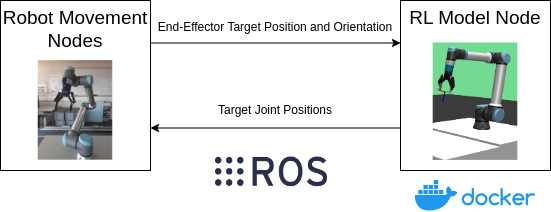
\includegraphics[width=\textwidth]{figs/ros_rl_flow.png}}
    \caption{Reinforcement Learning Integration with ROS}
    \label{fig:ros_rl_flow}
\end{figure}

This solution only replaces the computation of inverse or differential kynematics and still needs to be improved to not only completely replace MoveIt! but also to allow for real-time feedback, which would require a model capable of starting from different robot states.
